\documentclass{journal}
\usepackage{graphicx}
\usepackage{siunitx}
\usepackage{caption}
\usepackage{float}

\begin{document}
\title{AP Calculus Final Project}
\author{Joshua Morin-Baxter, Alan Zhu, Nathan Wiley, and George Hong}
\date{\today}

\maketitle

\begin{abstract}
This is an analysis of data taken from the GOSH Flight Path Predictor\textsuperscript{TM}.
Four separate sets of data were analyzed:
temperature vs. density, wind velocity vs. pressure, wind angle vs. wind velocity, and wind velocity vs. altitude.
Each is discussed in more depth in subsequent parts.
\end{abstract}

\part{Wind Velocity vs. Altitude}
This data seems to have two points that are of great interest.
\begin{figure}[h]
\centering
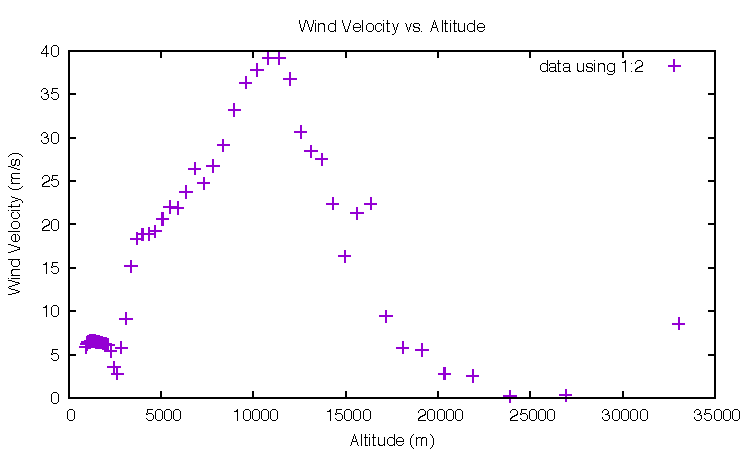
\includegraphics{josh-images/figure1.pdf}
\caption{Test}

\end{figure}


\part{Temperature Vs. Density}

\part{Wind Velocity vs. Pressure}
\begin{figure}[H]
\centering
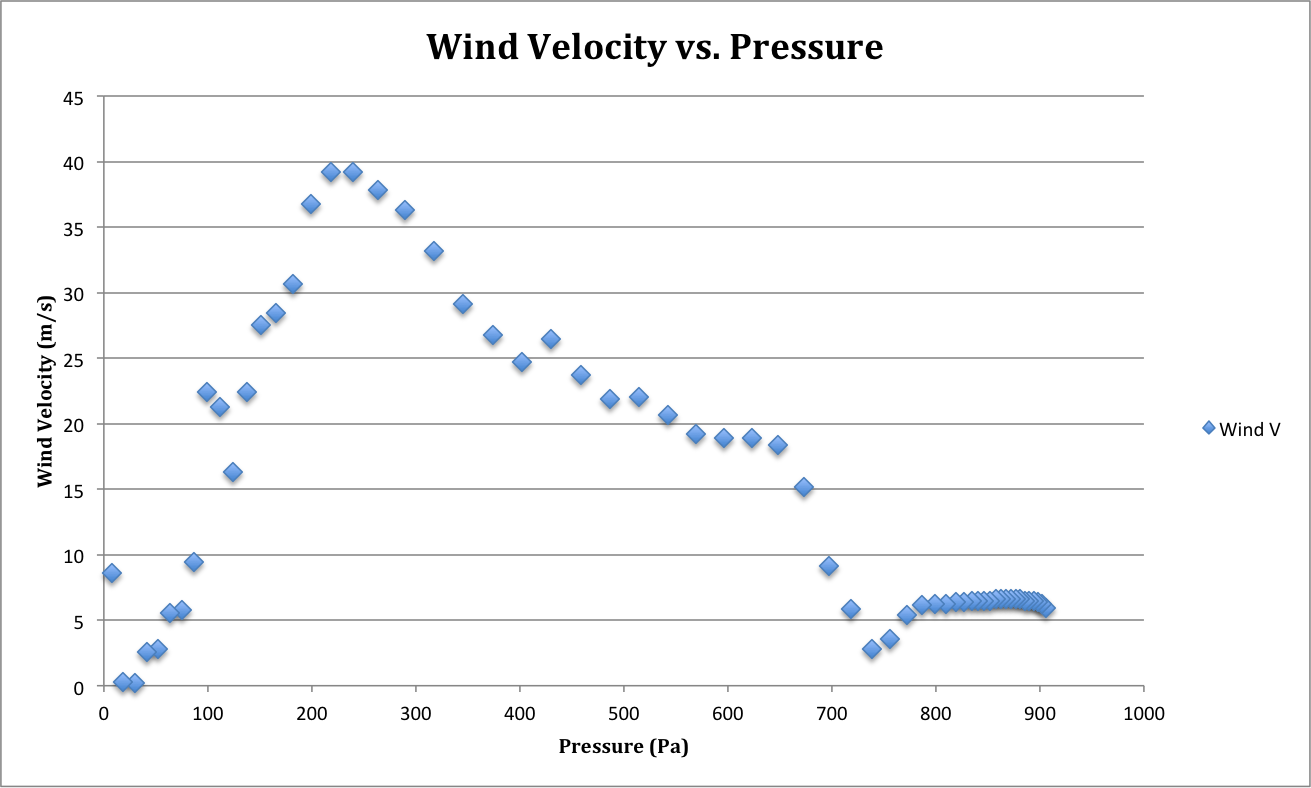
\includegraphics[width=5in]{IMG1CDATA.png}
\caption{Plot of Wind Velocity vs. Pressure}
\end{figure}

\begin{flushleft}
\textbf{Analysis:} After plotting all the points in a scatterplot, we notice our predicted concavities are well matched.  From the first derivative, we can split the data points into two distinct sections.  Pressures $\in$ [0,230) experience mostly increasing wind velocity, and Pressures $\in$ (230,725] experience primarily decreasing wind velocity.  Following a pressure of 800 Pascals, wind velocity stabilizes at $6.3\frac{m}{s} \pm 0.2\frac{m}{s}$.  We notice that wind speed is caused by shifts from high to low pressures, and the data from (230, 900) conforms to this principle: Wind speed increases as Pressure decreases.  Factors including temperature and the location of Jet Streams will result in divergence from this pattern.  Pressure is highest when altitude is lower, so the stable plateau of wind velocity at the highest pressures are expected.  Pressure collected in our data monotonically decreased with altitude.  Plots of Wind Velocity vs. Pressure or Altitude will simply be a horizontal reflection in this case.  
\end{flushleft}
\part{Wind Angle vs. Wind Velocity}



\end{document}
